\documentclass[12pt]{article}
\usepackage{epsfig}
\usepackage{graphicx}
\usepackage{a4}
\usepackage{amsmath}
\usepackage{latexsym}
\usepackage{cite}
%\usepackage{draftwatermark}
\usepackage{lineno}
\usepackage{xspace}
%\usepackage{chngcntr}


\usepackage{color}
\usepackage{colordvi}

\graphicspath{{Pics/}}
\DeclareGraphicsExtensions{.eps,.ps}

\textheight 22.0cm \textwidth 16.5cm
\oddsidemargin -0.1cm \evensidemargin -0.1cm

\usepackage{pslatex}
\usepackage[latin1]{inputenc}
\usepackage[T1]{fontenc}
\usepackage{amssymb}
\usepackage{url}

\newcommand{\msbar}{$\overline{\text{MS}}\, $\xspace}

%
\linenumbers
%
% ----------------------------------------------------------------------------------------------
%
\begin{document}

\begin{titlepage}
\noindent
Draft 1.0  \hfill 24 July 2019\\
\\
DESY AA-BBB %\hfill  2019\\
\\

\vspace{1.3cm}

\begin{center}
  {\bf 

\large

Extraction of parton distribution functions using recent LHCb and ALICE heavy-flavour measurements
  }
  \vspace{1.5cm}

  {\large
    PROSA Collaboration
  }\\

  \vspace{1.2cm}

\end{center}
 %\input{authors.tex}  
  \vspace{2.4cm}
\begin{center}
\large
{\bf Abstract}
\vspace{-0.2cm}
\end{center}
%%
The impact of recent measurements of heavy-flavour production in deep inelastic ep scattering and
in pp collisions on parton distribution functions is studied in a QCD analysis at next-to-leading order. 
Recent combined results of inclusive and heavy-flavour production cross sections in deep inelastic scattering at HERA are 
investigated together with heavy-flavour production measurements at the LHC. Differential cross sections of charm- and 
beauty-hadron production measured by the LHCb collaboration at the center of mass energies of 5, 7 and 13 TeV as well 
as the measurements of the ALICE experiment at the center of mass energies of 5 and 7 TeV are explored. 
These data impose additional constraints on the gluon and the sea-quark distributions at low partonic fractions
$x$ of the proton momentum, down to $x\approx10^{-6}$, which is the kinematic region of relevance for high-energy 
neutrino production. The impact of the resulting uncertainties in the nucleon composition, affecting predictions for 
the atmospheric prompt neutrino fluxes is presented.

%%
\vfill
\end{titlepage}


%
% ----------------------------------------------------------------------------------------------
%
\newpage

\section{Introduction}
\label{sect:intro}

The fundamental structure of the nucleon is described by the theory of strong interactions, quantum chromodynamics (QCD).
In the collinear factorisation, the nucleon structure is expressed in terms of parton distribution functions (PDFs), defined 
as probability densities for parton to carry $x$ fraction of the nucleon momentum at a factorisation scale $\mu_f$. While the 
scale evolution of the PDFs is calculated in perturbative QCD (pQCD) and presented by the DGLAP equations~\cite{Dokshitzer:1977sg,Gribov:1972ri,Altarelli:1977zs,Curci:1980uw,Furmanski:1980cm,Moch:2004pa,Vogt:2004mw}, the 
$x$-dependence must be constrained using the experimental measurements. The constraining power of experimental data 
on particular parton distribution is to large extent defined by the acceptance of the experiment. Measurements of 
neutral current (NC) and charged current (CC) cross sections in deep inelastic scattering (DIS) at HERA probe the $x$-range of $10^{-4}<x<10^{-1}$ and impose most significant constraints on the light quark PDFs and probe the gluon distribution via scaling violations. Additional constraints on flavour separation of the quark sea and on the gluon distribution at low and high $x$ are obtained by using the measurements at fixed target experiments and in proton-(anti)proton collisions. Heavy-flavour production in proton-proton collisions at the LHC is dominated by the gluon-gluon fusion, therefore corresponding measurements probe the gluon distribution directly. The measurements of forward charm~\cite{Aaij:2013mga} and beauty~\cite{Aaij:2013noa} production by the LHCb experiment at the center-of-mass energy $\sqrt{s}=7$ TeV were used for the first time by the PROSA collaboration~\cite{Zenaiev:2015rfa} to improve constraints on the gluon distribution at $5 \times 10^{-6}< x < 10^{-4}$, in the region not covered by any other data to that date. The resulting PDFs were further used to investigate the uncertainties in the predictions of prompt neutrino fluxes in the atmosphere~\cite{Garzelli:2016xmx}.       

Recent improvements in precision of HERA measurements, new experimental data on heavy flavour production at the LHC at 
different $\sqrt{s}$, together with new developments in the theory and improvements of the phenomenological tools, offer 
possibilities for stronger constraints on the gluon distribution at low $x$. These improvements in experimental measurements 
and the theory are explored in the QCD analysis presented in this paper, which updates the earlier result~\cite{Zenaiev:2015rfa}. The results are used in the predictions for the prompt atmospheric neutrino fluxes. 


\section{Input data sets and used theory predictions}
\label{sec:qcdanalysis}

The main objective of the present QCD analysis is to demonstrate the constraining power of the updated measurements of 
heavy-flavour production in DIS and proton-proton collisions for the determination of the PDFs of the proton. 
The QCD analysis is performed at next-to-leading order (NLO) using the xFitter framework~\cite{Alekhin:2014irh}. 
The updated combinations of the inclusive DIS cross sections~\cite{Abramowicz:2015mha} and of charm and beauty production cross sections~\cite{H1:2018flt} are used together with the measurements of charm and beauty hadroproduction in proton-proton scattering at the LHC. The latter include the measurements of charm hadroproduction by the LHCb collaboration at 5 TeV~\cite{Aaij:2016jht}, 7 TeV~\cite{Aaij:2013mga} and 13 TeV~\cite{Aaij:2015bpa}, and by ALICE at 5 TeV~\cite{Acharya:2019mgn} and 7 TeV~\cite{Acharya:2017jgo}. The measurements of beauty hadroproduction by the LHCb at 7 TeV~\cite{Aaij:2013noa} are also used.

The cross sections measured by the LHCb and ALICE in each $p_T$ range are normalized in rapidity $y$, $\frac{{\rm d}^2\sigma}{{\rm d}y{\rm d}p_T} / (\frac{{\rm d}^2\sigma}{{\rm d}y{\rm d}p_T})_{0}$. Here, $\left(\frac{{\rm d}^2\sigma}{{\rm d}y{\rm d}p_T}\right)_{0}$ is the cross section in the central LHCb rapidity bin, $3 < y < 3.5$. 
Note that ALICE measurements at $|y| < 0.5$ are normalised to the LHCb cross section measurement in $3 < y < 3.5$. 
The advantage of using the normalised cross section, demonstrated in the earlier PROSA analysis~\cite{Zenaiev:2015rfa}, 
is a significant reduction of the scale dependence in the theoretical prediction,  while retaining the sensitivity to 
the PDFs. 

In the presented QCD analysis, bin-to-bin correlations in the input measurements are taken into account as described in the following. The treatment of correlated experimental uncertainties for the HERA data follows that of the original publications~\cite{Abramowicz:2015mha,H1:2018flt}.
 
The correlated uncertainties in the ALICE and LHCb measurements reported in original publications~\cite{Aaij:2016jht, Aaij:2013mga, Aaij:2015bpa, Acharya:2019mgn, Acharya:2017jgo, Aaij:2013noa} as single numbers in $p_T$ and $y$ bins 
are treated as fully correlated, and the uncorrelated uncertainties are obtained by subtracting the correlated ones from the 
total uncertainties, in quadrature. The systematic uncertainties, reported as error intervals, see e.g. Table~(2) of ~\cite{Aaij:2016jht}, are assumed uncorrelated, since no details about their size in individual $p_T$ and $y$ bins are provided. 
Because of this treatment of systematics, most of the correlated systematic uncertainties cancel in the calculation of the normalised cross sections. In particular, a complete cancellation in the ratios of LHCb cross sections takes place.
For different final state measurements within one experiment, the tracking and luminosity uncertainties are treated as correlated. 
Furthermore, all experimental uncertainties are treated as uncorrelated among measurements at different center-of-mass energies. 
% and no further assumptions on the correlation of systematic uncertainties for different measurements are needed.
%Uncertainties in the branching ratios for the same channel are treated as correlated between different measurements. 
The uncorrelated uncertainties in the normalized cross sections $\frac{{\rm d}\sigma}{{\rm d}y_0}$ are propagated as correlated uncertainties to the respective complementary rapidity bins.
It is worthwhile to note, that the details of the experimental uncertainties and their correlations in each individual kinematic range is of great importance for the correct interpretation of the data.

In the presented QCD analysis, the scale evolution of partons is calculated through DGLAP equations at NLO, as implemented in 
the QCDNUM programme~\cite{openqcdrad}.  
The inclusion of small $x$ resummation which was shown to stabilise the perturbative expansion at next-to-next-to-leading order (NNLO) and improve the description of HERA data in PDF fits~\cite{Ball:2017otu,Abdolmaleki:2018jln} is left for future analyses, once all necessary theoretical ingredients become available.

The theoretical FFNS predictions for the HERA data are obtained using OPENQCDRAD~\cite{openqcdrad} code in the 
fixed-flavour-number scheme (FFNS) with the three active flavours in the proton, following the Ref.~\cite{H1:2018flt}. 
Similar to the earlier PROSA analysis~\cite{Zenaiev:2015rfa}, the theoretical predictions for the fully differential 
heavy-quark hadroproduction in proton-proton collisions, available at NLO in FFNS, are used. These are calculated using 
the MNR code, with the single-particle inclusive distributions computed using the pole mass scheme for the heavy quarks, 
and translated into the \msbar scheme expressions following the Ref.~\cite{Dowling:2013baa}. The \msbar mass scheme is 
then consistently used in the calculations for all used processes.

The factorisation and renormalisation scales are chosen to be $Q$ for the inclusive DIS, and $\mu_r = \mu_f = \sqrt{Q^2 + 4m_Q(m_Q)^2}$ for the heavy quark production in DIS, respectively, with $m_Q(m_Q)$ representing the heavy-quark mass in the \msbar scheme. 
For heavy quark production in proton-proton collision, $\mu_r = \mu_f = \sqrt{4m_Q(m_Q)^2+p_T^2}$ is assumed. 

The calculations for the heavy quark hadroproduction are supplemented with phenomenological non-perturbative fragmentation 
functions to describe the transition of heavy quarks into hadrons. The fragmentation of charm quarks into D-mesons is 
described by the Kartvelishvili function with $\alpha_K = 4.4 \pm 1.7$ as measured at HERA~\cite{Aaron:2008ac,Chekanov:2008ur}, 
and for the fragmentation of beauty quarks $\alpha_K = 11 \pm 3$ is used as measured at LEP~\cite{Nason:1999zj}, following 
the previous PROSA analysis~\cite{Zenaiev:2015rfa}.

The main QCD analysis is performed in the FFNS and the sensitivity of the heavy quark measurements to the PDFs and to the masses 
of the charm and beauty quarks is fully explored by treating $m_c(m_c)$ and $m_b(m_b)$ as free parameters in the fit.
The fit is also performed in the variable flavour number scheme (VFNS) to allow for possible applications of the 
results in the LHC analyses, e.g. tuning of the underlying event in the Monte Carlo simulations.


\section{PDF parametrisation}
\label{sec:pdfparam}

The PDFs are parametrised at the starting evolution scale of $\mu^2_{f0} = 1.9$~GeV$^2$, similar as in Ref.~\cite{Abramowicz:2015mha} and Ref.~\cite{Bonvini:2019wxf}, as follows:
\begin{equation}\begin{aligned}
xg(x) &= A_{g} x^{B_{g}}\,(1-x)^{C_{g}}\, (1 + F_{g} {\log x}),\\
u_\mathrm{v}(x) &= A_{u_\mathrm{v}}x^{B_{u_\mathrm{v}}}\,(1-x)^{C_{u_\mathrm{v}}}\,(1+E_{u_\mathrm{v}}x^2) ,\\
d_\mathrm{v}(x) &= A_{d_\mathrm{v}}x^{B_{d_\mathrm{v}}}\,(1-x)^{C_{d_\mathrm{v}}},\\
x\overline{\mathrm{U}}(x)&= A_{\overline{\mathrm{U}}}x^{B_{\overline{\mathrm{U}}}}\, (1-x)^{C_{\overline{\mathrm{U}}}}\, (1+D_{\overline{\mathrm{U}}}x), \\
x\overline{\mathrm{D}}(x)&= A_{\overline{\mathrm{D}}}x^{B_{\overline{\mathrm{D}}}}\, (1-x)^{C_{\overline{\mathrm{D}}}}.
\end{aligned}
\label{eq:dv}
\end{equation}

Here, $xg(x)$, $xu_{\mathrm{v}}(x)$ and $xd_{\mathrm{v}}(x)$ represent the gluon, up and down valence quark distributions, respectively. The sea quark distribution is defined as $x\Sigma(x)=x\overline{u}(x)+x\overline{d}(x)+x\overline{s}(x)$, with $x\overline{u}(x)$, $x\overline{d}(x)$, and $x\overline{s}(x)$ denoting the up, down, and strange antiquark distributions, respectively.
For the up- and down-type antiquark distributions, $x\overline{\mathrm{U}}(x)$ and $x\overline{\mathrm{D}}(x)$, relations $x\overline{\mathrm{U}}(x) = x\overline{u}(x)$ and $x\overline{\mathrm{D}}(x) = x\overline{d}(x) + x\overline{s}(x)$  are assumed.
The normalisation parameters $A_{u_{\mathrm{v}}}$, $A_{d_\mathrm{v}}$, and $A_{g}$ are determined by the QCD sum rules.
The strangeness fraction $f_{s} = x\overline{s}/( x\overline{d} + x\overline{s})$ is fixed to
$f_{s}=0.4$ as in the HERAPDF2.0 analysis~\cite{Abramowicz:2015mha}.
Additional constraints $B_{\overline{\mathrm{U}}} = B_{\overline{\mathrm{D}}}$ and $A_{\overline{\mathrm{U}}} = A_{\overline{\mathrm{D}}}(1 - f_{s})$ are imposed to ensure the same normalisation for the $x\overline{u}$ and $x\overline{d}$ distributions as $x \to 0$.
The term $F_g\log x$ was proposed in~\cite{Bonvini:2019wxf} to provide a more flexible functional form at low $x$.

The predicted and measured cross sections together with their corresponding uncertainties are used to build a global $\chi^2$, minimized to determine the initial PDF
parameters. The $\chi^2$ definition follows that of Eq.~(32) in Ref.~\cite{Abramowicz:2015mha}. In the minimisation, performed 
using the MINUIT package~\cite{James:1975dr}, the experimental uncertainties in the heavy-quark normalised cross 
sections are treated as additive, and the treatment of the experimental uncertainties for the HERA DIS data follows 
the prescription given in Ref.~\cite{Abramowicz:2015mha}.

The parameters in Eq.(\ref{eq:dv}) are selected by first parametrising each PDF as
\begin{equation}
xf(x) = Ax^B(1-x)^C(1+Dx+Ex^2)
\label{eq:de}
\end{equation}
with all D and E parameters set to zero. The other 
parameters are then included in the fit one at a time. The improvement in $\chi^2$ of the fits is monitored and the 
procedure is stopped when no further improvement is observed. The inclusion of the $F_{g}$ parameter does not lead to sizable change in $\chi^2$, in particular, its fitted value is consistent with $0$ within uncertainty, however the variation of $F_{g}$ significantly affects the fit uncertainties.
To ensure that the gluon PDF at low $x$ is not overconstrained in the fit, different functional forms in the parametrisation were tested, as used in the ABMP16~\cite{Alekhin:2017kpj}, CT14~\cite{Dulat:2015mca}, HERAPDF2.0~\cite{Abramowicz:2015mha}, MMHT2014~\cite{Harland-Lang:2014zoa} and Bonvini-Giuli (BG)~\cite{Bonvini:2019wxf} PDF fits. The details of this study are given in Appendix (Section~\ref{sec:gluonpar}).


\section{PDF uncertainties}
\label{sec:pdfunc}

The PDF uncertainties are investigated according to the general approach of HERAPDF2.0 analysis~\cite{Abramowicz:2015mha}, with the fit, model, and parametrisation uncertainties taken into account.

The fit uncertainties arising from the uncertainties in the measurements are estimated by using the Hessian method~\cite{Pumplin:2001ct}, adopting the tolerance criterion of $\Delta \chi^2$ = 1 and correspond to 68\% confidence level.

To investigate the impact of model assumptions on the resulting PDFs, alternative fits are performed and the differences to the central result are considered as model uncertainties. The strangeness fraction is varied as $0.3 \leq f_{s} \leq 0.5$ and the value of $Q^2_{\text{min}}$ imposed on the HERA data as $2.5 \leq Q^2_\textrm{min}\leq 5.0\textrm{GeV}^2$. The FFNS strong coupling constant is assumed as $0.105 < \alpha_s^{n_f=3}(M_Z) < 0.107$ (corresponding to the VFNS values of $0.117 < \alpha_s^{n_f=5}(M_Z) < 0.119$~\cite{Tanabashi:2018oca}). The variation of the fragmentation parameters $\alpha_K = 4.4 \pm 1.7$ for charm hadrons and $\alpha_K = 11 \pm 3$ for beauty hadrons is performed.
The scales $\mu_f$ and $\mu_r$ for heavy quark production are varied independently and simultaneously up and down by a factor of two, excluding variations of the two scales in opposite directions. Note that for 
the normalized cross section predictions, the simultaneous variation of the $\mu_f$ and $\mu_r$ scales in the same direction results in the largest deviation in the 
resulting PDFs and is considered as one PDF uncertainty eigenvector.

The parametrisation uncertainty is estimated by extending the functional form of each PDF in Eq.~(\ref{eq:dv}) with additional parameters $D$ and $E$ (see Eq.~\ref{eq:de}), 
which are added or removed one at a time and do not impact the $\chi^2$. 
In particular, the shape of the gluon PDF is extended by adding the $+G_g\log^2 x$ term~\cite{Bonvini:2019wxf}. This modification does not result in an improvement in $\chi^2$ and therefore is not considered in the nominal parametrisation. 
The variation of the starting scale, $1.6 < \mu_\mathrm{f0}^2 < 2.2$~GeV$^2$, is also taken into account as contribution to the parametrisation uncertainty. The parametrisation uncertainty is constructed as an envelope built from the maximal differences between the PDFs resulting from all the parameterization variations and the central fit at each x value.

The total PDF uncertainty is obtained by adding experimental, model, and parameterization  uncertainties in quadrature.

\section{Results}
\label{sec:results}

The quality of the overall fit can be judged based on the global $\chi^2$ divided
by the number of degrees of freedom, $n_{dof}$. For each data set included in the fit, a partial $\chi^2$
divided by the number of measurements (data points), $n_{dp}$, is provided. The correlated part of $\chi^2$
quantifies the influence of the correlated systematic uncertainties in the fit. The global and partial $\chi^2$ values 
for each data set are listed in Table~\ref{tab:chi}, illustrating a general agreement among all the data sets. 
The central values and the uncertainties of the fitted parameters are given in Table~\ref{tab:pars}.

\begin{table}
\renewcommand*{\arraystretch}{1.12}
\tabcolsep1cm
    \centering
\begin{tabular}{ll}
    Dataset & $\chi^2/\textrm{ndp}$ \\
    \hline
    HERA CC $e^{+}p$ & 62 / 39  \\ 
    HERA CC $e^{-}p$ & 49 / 42  \\ 
    HERA NC $e^{-}p$ & 227 / 159  \\ 
    HERA NC $e^{+}p$ 820 GeV & 68 / 70  \\ 
    HERA NC $e^{+}p$ 920 GeV & 440 / 377  \\ 
    HERA NC $e^{+}p$ 460 GeV & 223 / 204  \\ 
    HERA NC $e^{+}p$ 575 GeV & 223 / 254  \\ 
    HERA NC charm & 49 / 52  \\ 
    HERA NC beauty & 18 / 27  \\ 
    LHCb 7 TeV $B^0$ & 52 / 76  \\ 
    LHCb 7 TeV $B^{+}$ & 129 / 108  \\ 
    LHCb 7 TeV $B^{0}_s$ & 37 / 60  \\ 
    LHCb 7 TeV $D^0$ & 15 / 30  \\ 
    LHCb 7 TeV $D^{+}$ & 19 / 29  \\ 
    LHCb 7 TeV $D^{+}_{s}$ & 14 / 20  \\ 
    LHCb 7 TeV $D^{*+}$ & 16 / 22  \\ 
    LHCb 5 TeV $D^0$ & 60 / 35  \\ 
    LHCb 5 TeV $D^{+}$ & 25 / 35  \\ 
    LHCb 5 TeV $D^{+}_{s}$ & 30 / 29  \\ 
    LHCb 5 TeV $D^{*+}$ & 35 / 30  \\ 
    LHCb 13 TeV $D^0$ & 111 / 60  \\ 
    LHCb 13 TeV $D^{+}$ & 72 / 64  \\ 
    LHCb 13 TeV $D^{+}_{s}$ & 69 / 55  \\ 
    LHCb 13 TeV $D^{*+}$ & 82 / 54  \\ 
    ALICE 7 TeV $D^0$ & 5.1 / 8  \\ 
    ALICE 7 TeV $D^{+}$ & 0.75 / 7  \\ 
    ALICE 7 TeV $D^{*+}$ & 2.3 / 6  \\ 
    ALICE 5 TeV $D^0$ & 6.3 / 10  \\ 
    ALICE 5 TeV $D^{+}$ & 5.8 / 9  \\ 
    ALICE 5 TeV $D^{+}_{s}$ & 2.5 / 4  \\ 
    ALICE 5 TeV $D^{*+}$ & 1.7 / 9  \\ 
    \hline
    Correlated $\chi^2$  & 282  \\ 
    Log penalty $\chi^2$  &  -32  \\ 
    \hline
    %\rowcolor{white}
    %\midrule
    Total $\chi^2$ / dof  & 2401 / 1969  \\ 
    %\rowcolor{white}
    %\midrule
    %$\chi^2$ p-value  & 0.00 & 0.00   \\ 
    %\bottomrule
\end{tabular}
\caption{The global and partial $\chi^2$ values for each data set together with the corresponding number of data points (ndp). The correlated $\chi^2$ and the log penalty $\chi^2$ entries refer to the $\chi^2$ contributions from the correlated uncertainties and from the logarithmic term, respectively, as described in Ref.~\cite{Abramowicz:2015mha}.}
\label{tab:chi}
\end{table}

\begin{table}
    \renewcommand*{\arraystretch}{1.12}
    \tabcolsep1cm
    \centering
\begin{tabular}{ll}
    Parameter & Value \\
    \hline
    $B_g$ & $0.004 \pm 0.053$  \\
    $C_g$ & $6.25 \pm 0.29$  \\
    $Fg$ & $0.068 \pm 0.024$  \\
    $B_{u_v}$ & $0.644 \pm 0.030$  \\
    $C_{u_v}$ & $4.862 \pm 0.076$  \\
    $E_{u_v}$ & $15.8 \pm 2.2$  \\
    $B_{d_v}$ & $0.873 \pm 0.076$  \\
    $C_{d_v}$ & $4.61 \pm 0.35$  \\
    $C_{\overline{U}}$ & $7.36 \pm 0.77$  \\
    $D_{\overline{U}}$ & $10.1 \pm 2.4$  \\
    $A_{\overline{D}}$ & $0.1061 \pm 0.0058$  \\
    $B_{\overline{D}}$ & $-0.1661 \pm 0.0062$  \\
    $C_{\overline{D}}$ & $12.7 \pm 3.0$  \\
    $m_c(m_c)$ & $1.230 \pm 0.031$ GeV  \\
    $m_b(m_b)$ & $3.977 \pm 0.100$ GeV  \\
\end{tabular}
\caption{The resulting parameters for the PDFs with their fit uncertainties.}
\label{tab:pars}
\end{table}

The fitted PDFs with their total uncertainties at the scale $\mu^2_f=10$ GeV$^2$ are shown in Fig.~\ref{fig:pdfs}. These are compared to the result of the PROSA 2015 fit~\cite{Zenaiev:2015rfa}. In Fig.~\ref{fig:pdfratios} (left), the gluon distribution 
normalised to the one from the PROSA 2015 fit is shown. The two results are in a very good agreement and a significant improvement 
in the precision of the gluon PDF is achieved at $x < 10^{-4}$, as compared to the PROSA 2015 fit. 
The valence and sea quark PDFs are in good agreement with the result of HERAPDF2.0 analysis~\cite{Abramowicz:2015mha} and the 
observed differences in these distributions to the PROSA 2015 analysis are attributed to the update of the DIS measurements~\cite{Aaron:2009aa} used in Ref.~\cite{Zenaiev:2015rfa} to the final combination~\cite{Abramowicz:2015mha} of the HERA data.

The relative total, fit, model and parametrisation uncertainties for the gluon PDF are shown in Fig.~\ref{fig:pdfratios} (right). 
The total uncertainties are dominated by the model uncertainties, with the largest contributions arising from the scale 
variations in predictions for heavy-quark hadroproduction. Reduction of these uncertainties would require theoretical calculations at higher order.

\begin{figure}
    \centering
    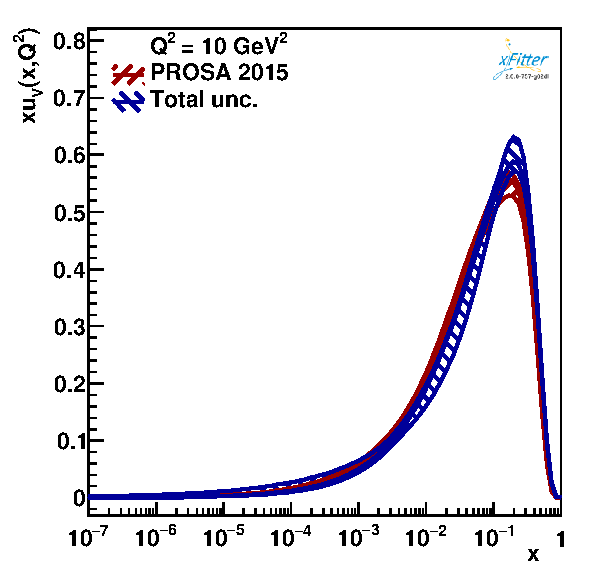
\includegraphics[width=0.49\textwidth]{figs/q2_10_pdf_uv.pdf}
    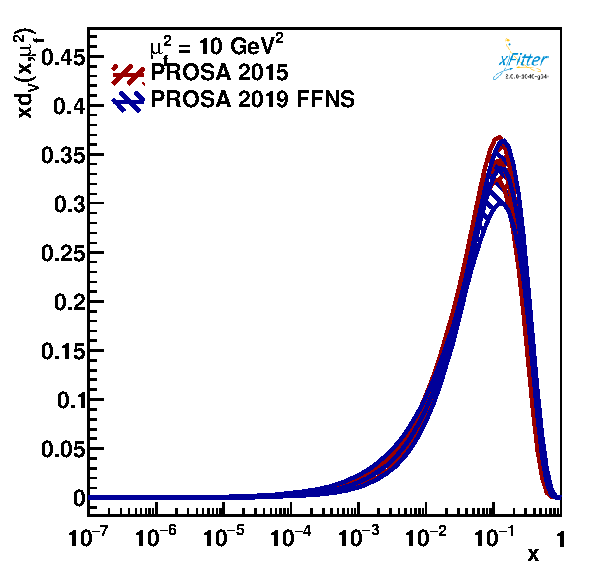
\includegraphics[width=0.49\textwidth]{figs/q2_10_pdf_dv.pdf}\\
    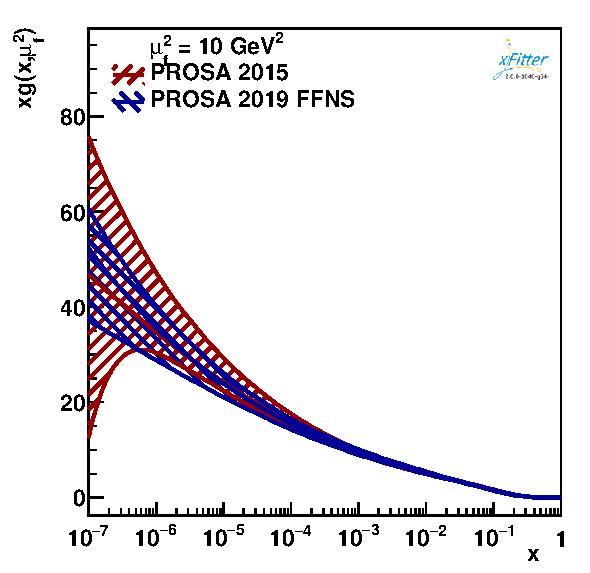
\includegraphics[width=0.49\textwidth]{figs/q2_10_pdf_g.pdf}
    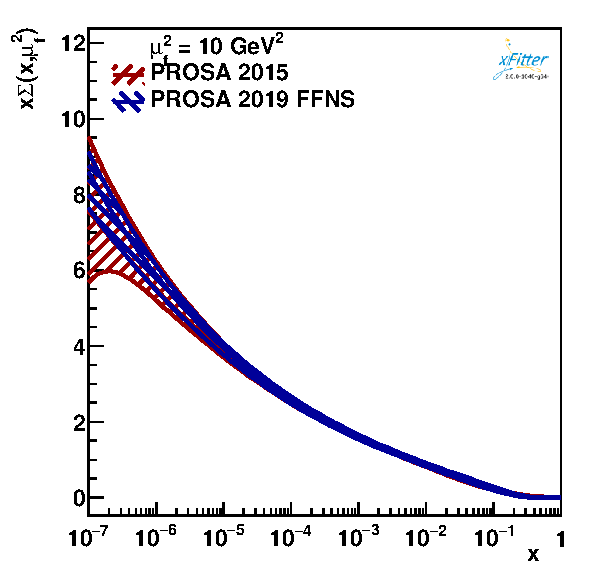
\includegraphics[width=0.49\textwidth]{figs/q2_10_pdf_Sea.pdf}
    \caption{The fitted PDFs with their total uncertainties at the scale $\mu^2_f=10$ GeV$^2$ compared with the distributions from the PROSA 2015 fit.}
    \label{fig:pdfs}
\end{figure}

\begin{figure}
    \centering
    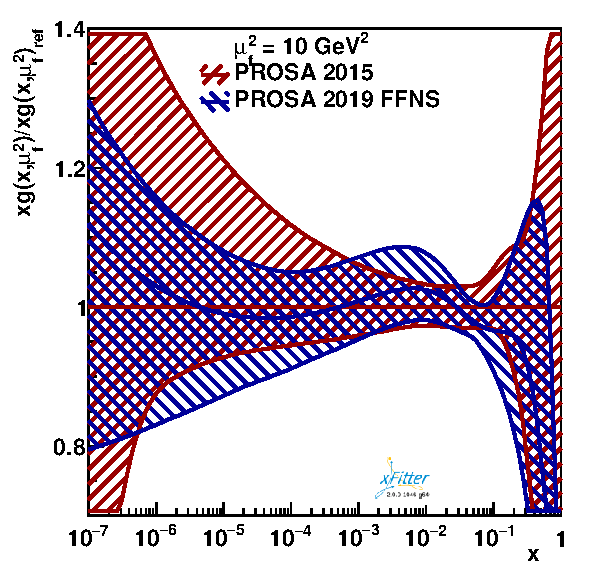
\includegraphics[width=0.49\textwidth]{figs/q2_10_pdf_g_ratio.pdf}
    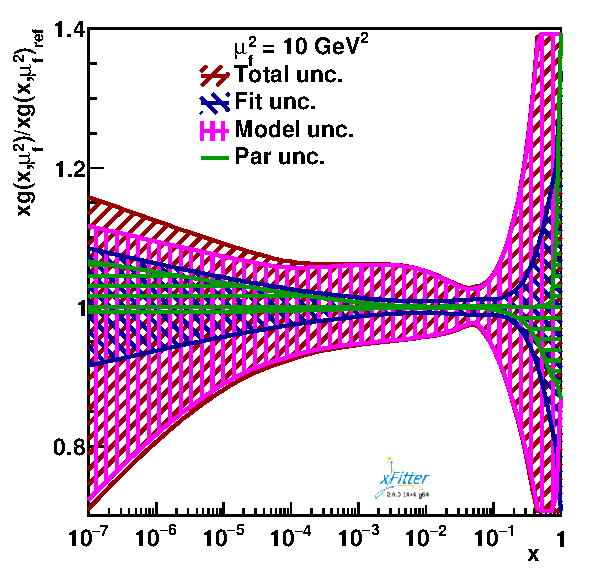
\includegraphics[width=0.49\textwidth]{figs/gluonunc.pdf}
    \caption{(left) The gluon PDF with their total uncertainties at the scale $\mu^2_f=10$ GeV$^2$ divided by the gluon PDF from the PROSA 2015 fit. (right) The relative total, fit, model and parametrisation uncertainties for the gluon PDF at the scale $\mu^2_f=10$ GeV$^2$.}
    \label{fig:pdfratios}
\end{figure}

The resulting PDFs are available in the LHAPDF format at [\dots] in both FFNS and VFNS.
The performance of the new PDFs presented here was tested by computing predictions for the inclusive and multi-jet production in DIS~\cite{Chekanov:2002be,Chekanov:2006xr,Abramowicz:2010cka,Aktas:2007aa,Aaron:2010ac} and jet~\cite{Chatrchyan:2012bja} and top quark-antiquark production~\cite{Sirunyan:2017azo,Sirunyan:2019zvx} in proton-proton collisions. The VFNS variant of the presented PDFs is used. The results are found similar to those using HERAPDF2.0 PDF.%
\footnote{The resulting predictions compared to the measurements by H1, ZEUS and CMS experiments will be put on the PROSA webpage for reference.}


\section{Predictions for prompt atmospheric neutrino fluxes}
\label{sec:astro}

\section{Summary}
\label{sec:summary}

\section*{Acknowledgments}

We would like to thank I.~Novikov and A.~Glazov for their help with developing and using new features of the xFitter framework, and V.~Bertone for his help with the APFEL library.
The work of O.~Z. has been supported by Bundesministerium f\"ur Bildung und Forschung (contract 05H18GUCC1).

%%%%%%%%%%%%%%%%%%%%%%%%%%%%%%%%%%%%%%%%%
%%%%%%%%%%%%%%%%%%%%%%%%%%%%%%%%%%%%%%%%%

\bibliographystyle{spphys}
\bibliography{prosa2019,extra}

\clearpage
\appendix

\section{Additional studies of gluon parametrisation}
\label{sec:gluonpar}

To ensure that the gluon PDF at low $x$ is not overconstrained in the fit, different functional forms in the parametrisation 
are tested, as used in the ABMP16~\cite{Alekhin:2017kpj}, CT14~\cite{Dulat:2015mca}, HERAPDF2.0~\cite{Abramowicz:2015mha} and Bonvini-Giuli (BG)~\cite{Bonvini:2019wxf} PDF fits:

\begin{equation}
\begin{aligned}
\textrm{ABMP16:}~~~~~~ &xg(x)=A (1 - x)^b x^{a (1 + \gamma_{1} x)},\\
\textrm{CT14:}~~~~~~ &xg(x) = Ax^{a_1}(1-x)^{a_2}(e_0(1-y)^2+e_1(2y(1-y))+y^2), y=2\sqrt{x}-x,\\
%\textrm{MMHT2014:}~~~~~~ &xg(x) = Ax^B(1-x)^C(1+a_1y+a_2(2y^2-1))+A^{\prime}_gx^{B^{\prime}_g}(1-x)^{25}, y=1-2\sqrt{x},\\ 
\textrm{HERAPDF2.0:}~~~~~~ &xg(x)=A_gx^{B_g}(1-x)^{C_g}+A^{\prime}_gx^{B^{\prime}_g}(1-x)^{25},\\
\textrm{HERAPDF2.0 no flex. $g$:}~~~~~~ &xg(x)=A_gx^{B_g}(1-x)^{C_g},\\
\textrm{BG:}~~~~~~ &xg(x)=A_{g} x^{B_{g}}\,(1-x)^{C_{g}}\, (1 + F_{g} {\log x} + G_{g} {\log^2 x}),\\
\end{aligned}
\label{eq:gluonpar}
\end{equation}

These functional forms are characterised by $3$ (HERAPDF2.0 no flex. $g$), $4$ (ABMP16), $5$ (CT14, HERAPDF2.0, BG) or $7$ (MMHT2014) parameters controlling the gluon PDF (c.f.\ $4$ parameters in the presented nominal parametrisation of Eq.~\ref{eq:dv}). 
The resulting gluon distributions are presented in Fig.~\ref{fig:gluonpar}. The parametrisations of ABMP16, HERAPDF2.0 without the flexible gluon, and BG provide very similar results to that of the nominal parametrisation in Eq.~\ref{eq:dv}. 
Note that also the HERAPDF2.0 analysis considered the parametrisation without the flexible gluon, stamped it as `alternative' gluon parameterisation~\cite{Abramowicz:2015mha} and provided primarily for predictions of cross sections at very low $x$, such as very high-energy neutrino cross sections.

The fit using the HERAPDF2.0 and CT14 parametrisations yielded a gluon distribution with a sharp turnover to negative values 
at $x \sim 10^{-6}$, i.e.\ at the edge of the kinematic reach of the used measurements. Using such PDFs would 
lead to a negative prediction for the total charm hadroproduction cross sections at $\sqrt{s} \gtrsim 20$~TeV, similar to the observation of Ref.~\cite{Accardi:2016ndt}. Therefore these parametrisations are discarded (despite they provide an improved $\chi^2$, by $22$ and $7$ units when using the HERAPDF2.0 and CT14 parametrisations, respectively). In this analysis, it was not possible to achieve convergence of the fit using the MMHT2014 parametrisation~\cite{Harland-Lang:2014zoa}, because of no essential sensitivity of the used data sets to the gluon distribution at high $x$.

%The MMHT2014 parametrisation is similar to the one used in HERAPDF2.0 at low $x$, but has more flexibility at high $x$. 
%In the presented analysis, it was not possible to achieve convergence using the MMHT2014 parametrisation, because of not essential sensitivity of the used data sets to the gluon distribution at high $x$. However discarding parameters controlling 
%the high-$x$ behaviour would result in the HERAPDF2.0 parametrisation.

The gluon distribution obtained in the fit using different parametrisations (see Eq.~\ref{eq:gluonpar}) are shown on Fig.~\ref{fig:gluonpar}.

\begin{figure}
    \centering
    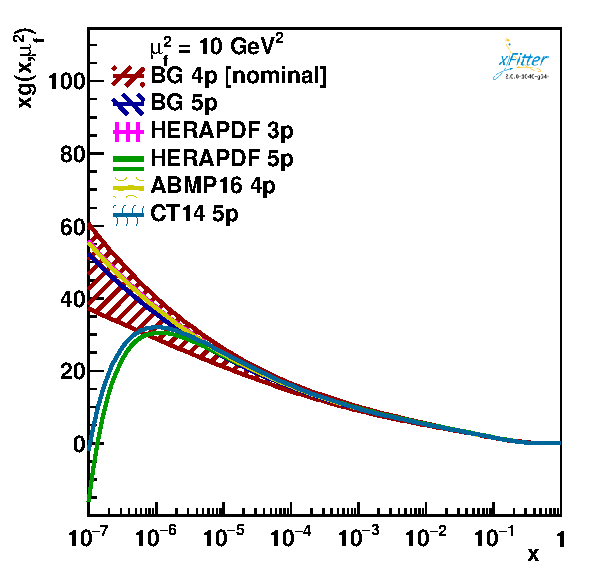
\includegraphics[width=0.49\textwidth]{figs/gluonpar/q2_10_pdf_g.pdf}
    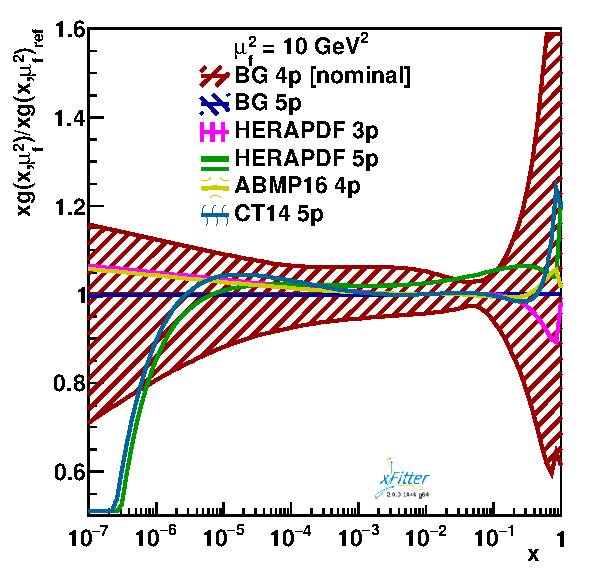
\includegraphics[width=0.49\textwidth]{figs/gluonpar/q2_10_pdf_g_ratio.pdf}
    \caption{(left) The gluon PDF with their total uncertainties at the scale $\mu^2_f=10$ GeV$^2$ obtained using different gluon parametrisations (see Eq.~\ref{eq:gluonpar}). (right) The same PDFs normalised to the distribution obtained using the nominal parametrisation.}
    \label{fig:gluonpar}
\end{figure}

\section{Fit in VFNS}
\label{sec:vfns}

The fit in the VFNS is performed using the APFEL library~\cite{Bertone:2013vaa} interfaced in xFitter.
The theoretical predictions for the HERA data are computed using the FONLL-B scheme~\cite{Forte:2010ta} with the pole charm and beauty quark masses set to $m_c^{\textrm{pole}} = 1.4$ GeV and $m_c^{\textrm{pole}} = 4.5$ GeV respectively.
However, no VFNS calculation for heavy-quark hadroproduction is interfaced to public tools and can be used for PDF fitting.
To keep using the MNR calculations with the VFNS, we exploit the feature of the APFEL library to choose arbitrary heavy-quark matching thresholds~\cite{Bertone:2017ehk}. These thresholds are set to values:
\begin{equation}
\begin{aligned}
\mu_c &= 4.5m_c^{\textrm{pole}} = 6.3~\textrm{GeV},\\
\mu_b &= 4.5m_b^{\textrm{pole}} =  20.25~\textrm{GeV}.
\label{eq:thr}
\end{aligned}
\end{equation}
We imposed kinematic cuts $p_T < 5$ GeV and $p_T < 16$ GeV on the LHC charm and beauty data, respectively, to ensure that we are working with not more than 3 (4) light flavours when calculating predictions for charm (beauty) data.
The strong coupling strength is set to $\alpha_s^{n_f = 5}(M_Z) = 0.118$~\cite{Tanabashi:2018oca}, while all other settings are the same as in the FFNS fit.
The specific matching thresholds in Eq.~\ref{eq:thr} are chosen to ensure that a sufficient amount of the LHC charm and beauty data is still included in the fit.
The choice of the matching thresholds is arbitrary and amounts to a renormalisation scheme choice~\cite{Bertone:2017ehk}, therefore we have verified that the fit results are stable under variations within $3.1 \le \mu_Q/m_Q^{\textrm{pole}} \le 6$, with the $p_T$ cuts on the charm and beauty LHC data modified accordingly.

In this fit, $\chi^2 = 2114$ is obtained for $n_{dof} = 1714$, indicating a similar quality of data description as compared to the fit in the FFNS.
The resulting PDFs are available in the LHAPDF format at [\dots]. No PDF uncertainties are provided with this set.

\if 0
\section{Additional plots}
\label{sec:extraplots}

%{\color{blue}(These plots provided on request of M.V.: do we want them in the paper?)}

The fitted PDFs with their total uncertainties at the starting scale of PDF evolution $\mu^2_f=1.9$~GeV$^2$ are shown in Fig.~\ref{fig:pdfs19}, superimposed with the PDFs from the PROSA 2015 fit~\cite{Zenaiev:2015rfa}.

\begin{figure}
    \centering
    \includegraphics[width=0.49\textwidth]{figs/{q2_1.9_pdf_uv}.pdf}
    \includegraphics[width=0.49\textwidth]{figs/{q2_1.9_pdf_dv}.pdf}\\
    \includegraphics[width=0.49\textwidth]{figs/{q2_1.9_pdf_g}.pdf}
    \includegraphics[width=0.49\textwidth]{figs/{q2_1.9_pdf_Sea}.pdf}
    \caption{The fitted PDFs with their total uncertainties at the scale $\mu^2_f=1.9$ GeV$^2$ compared with the distributions from the PROSA 2015 fit.}
    \label{fig:pdfs19}
\end{figure}
\fi

\end{document}


